%%%%%%%%%%%%%%%%%%%%%%%%%%%%%%%%%%%%%%%%%%%%%%%%
%% Compile: PDFLaTeX BibTeX PDFLaTeX PDFLaTeX
%% Course Slides: Wissenschaftliches Arbeiten
%% Antonio Machicao y Priemer
%%%%%%%%%%%%%%%%%%%%%%%%%%%%%%%%%%%%%%%%%%%%%%%%

\documentclass[a4paper,10pt, bibtotoc]{beamer}
%\documentclass[a4paper,10pt,handout]{beamer}

%%%%%%%%%%%%%%%%%%%%%%%%%
%% PACKAGES & COMMANDS 
%%%%%%%%%%%%%%%%%%%%%%%%%

%%%%%%%%%%%%%%%%%%%%%%%%%%%%%%%%%%%%%%%%%%%%%%%%%%%%
%%%          MyP-Packages   2018.12.08    XeLaTeX
%%%%%%%%%%%%%%%%%%%%%%%%%%%%%%%%%%%%%%%%%%%%%%%%%%%%


%\usepackage[utf8]{inputenc} %XeLaTeX

%% For German texts
\usepackage[ngerman,english]{babel}

%% For English texts
%\usepackage[ngerman,english]{babel}

%% Captions numbered in Beamer 
\setbeamertemplate{caption}[numbered]

%% Change ''Abbildung'' into ''Abb.'' 
%% for: babel
	\renewcommand{\thefigure}{\arabic{figure}}
	\addto\captionsngerman{%
		\renewcommand{\figurename}{Abb.}%
	}
	\renewcommand{\figurename}{Abb.} 

%% Change ''Figure'' into ''Fig.'' 
%% for: babel
	\renewcommand{\thefigure}{\arabic{figure}}
	\addto\captionsenglish{%
		\renewcommand{\figurename}{Fig.}%
	}
%	\renewcommand{\figurename}{Fig.} %% << not needed? 


%% TIPA encoding needs options: T3 & T1
\usepackage[T3,T1]{fontenc}  %not needed in XeLaTeX (?)

%\usepackage{fontspec} % XeLaTeX: Problem: Libertine+Fontspec+TIPA

%% Font
\usepackage{lmodern}
%\usepackage{libertine} % XeLaTeX: Problem: Libertine+Fontspec+TIPA

%% Blind text: \blindtext \Blindtext \blindtext[5] \blindlist{itemize}[x] ...
\usepackage{blindtext}

%% ulem: Strike out
\usepackage[normalem]{ulem}  

%% graphicx: if gb4e is active PDFLaTeX does not accept files with underline. PDFLaTeX accepts files only with .jpg, .png, .pdf endings
\usepackage{graphicx}

%% Math symbols
\usepackage{amsmath}
\usepackage{amsfonts}
\usepackage{amssymb}
\usepackage{MnSymbol} 				% Meaning brackets 

%% Toggles
\usepackage{etoolbox}
	\newtoggle{handout}


%%%%%%%%%%%%%%%%%%%%%%%%%%%%%%%%%%%%%%%%%%%%%%%%%%%%
%%%         Tables & Lists & Columns            
%%%%%%%%%%%%%%%%%%%%%%%%%%%%%%%%%%%%%%%%%%%%%%%%%%%%

% Text in columns: \begin{multicols}{n} \columnbreak \end{multicols}
\usepackage{multicol}
%	\setlength{\columnsep}{.5cm}	

%% Tables with specified width
\usepackage{tabularx}

%% For complex tables
\usepackage{array}

%% For other tables
\usepackage{booktabs}

%% For more than one row in a table
\usepackage{multirow}

%% Special lists: itemize*
\usepackage{mdwlist}


%%%%%%%%%%%%%%%%%%%%%%%%%%%%%%%%%%%%%%%%%%%%%%%%%%%%
%%%          Coloured elements                  
%%%%%%%%%%%%%%%%%%%%%%%%%%%%%%%%%%%%%%%%%%%%%%%%%%%%
%Use xcolor before `gb4e'!
\usepackage{xcolor}


%%%%%%%%%%%%%%%%%%%%%%%%%%%%%%%%%%%%%%%%%%%%%%%%%%%%
%%%          Trees                               
%%%%%%%%%%%%%%%%%%%%%%%%%%%%%%%%%%%%%%%%%%%%%%%%%%%%
%% Forest must be loaded before `gb4e'
\usepackage{forest}
	
	%% Needed for the "actual forest version"
	\useforestlibrary{linguistics}
	\forestapplylibrarydefaults{linguistics}

%% Old forest version
%\usepackage{etex}		%For Forest bug
%\usepackage{../forestold}
	
	
%%%%%%%%%%%%%%%%%%%%%%%%%%%%%%%%%%%%%%%%%%%%%%%%%%%%
%%%          Venndiagram                         
%%%%%%%%%%%%%%%%%%%%%%%%%%%%%%%%%%%%%%%%%%%%%%%%%%%%
%% Package needed: tikz
\usepackage{venndiagram}


%%%%%%%%%%%%%%%%%%%%%%%%%%%%%%%%%%%%%%%%%%%%%%%%%%%%%
%%%%          Verbatim                            
%%%%%%%%%%%%%%%%%%%%%%%%%%%%%%%%%%%%%%%%%%%%%%%%%%%%%
%%`Listings' must be loaded before `gb4', use `verbatim' otherwise
\usepackage{listings}

\lstset{
	language=TeX,
	backgroundcolor=\color{lightgray},
	basicstyle={\footnotesize\ttfamily\color{blue}},
	showstringspaces=false,
	columns=flexible
}
\lstset{literate=%
	{Ö}{{\"O}}1
	{Ä}{{\"A}}1
	{Ü}{{\"U}}1
	{ß}{{\ss}}2
	{ü}{{\"u}}1
	{ä}{{\"a}}1
	{ö}{{\"o}}1
}

%\lstset{%frame=tb,
%	language=Perl,
%	aboveskip=3mm,
%	belowskip=3mm,
%	showstringspaces=false,
%	columns=flexible,
%	basicstyle={\small\ttfamily\color{blue}},
%	numbers=none,
%	%numberstyle=\tiny\color{gray},
%	extendedchars=false,
%	morekeywords={foo},
%	otherkeywords={\#\#},
%	%keywordstyle=\color{blau},
%	%commentstyle=\color{whiteblue},
%	%stringstyle=\color{mauve},
%	breaklines=true,
%	breakatwhitespace=true,
%	tabsize=3
%}


%%%%%%%%%%%%%%%%%%%%%%%%%%%%%%%%%%%%%%%%%%%%%%%%%%%%%
%%%%       Attribute Value Matrices               
%%%%%%%%%%%%%%%%%%%%%%%%%%%%%%%%%%%%%%%%%%%%%%%%%%%%%
\usepackage{../../texfiles-beamer/avm}
%%% Setting of avm (see LSP Guidelines)
	%	\avmfont{\sc}
	%	\avmvalfont{\it}
	\avmfont{\normalfont \scshape} 
	\avmvalfont{\normalfont \itshape} 
%% command to fontify the type values of an avm 
	\newcommand{\tpv}[1]{{\avmjvalfont #1}} 
%% command to fontify the type of an avm and avmspan it
	\newcommand{\tp}[1]{\avmspan{\tpv{#1}}}


%%%%%%%%%%%%%%%%%%%%%%%%%%%%%%%%%%%%%%%%%%%%%%%%%%%%
%%%          IPA                                 
%%%%%%%%%%%%%%%%%%%%%%%%%%%%%%%%%%%%%%%%%%%%%%%%%%%%
%\usepackage[noenc,safe]{tipa}	%in PDFLaTeX
\usepackage[safe]{tipa}	% in XeLaTeX


%%%%%%%%%%%%%%%%%%%%%%%%%%%%%%%%%%%%%%%%%%%%%%%%%%%%
%%%          Vowel diagram                       
%%%%%%%%%%%%%%%%%%%%%%%%%%%%%%%%%%%%%%%%%%%%%%%%%%%%
%\usepackage{vowel}


%%%%%%%%%%%%%%%%%%%%%%%%%%%%%%%%%%%%%%%%%%%%%%%%%%%%
%%%          Bibliography                        
%%%%%%%%%%%%%%%%%%%%%%%%%%%%%%%%%%%%%%%%%%%%%%%%%%%%
\usepackage{natbib}	
	\setcitestyle{notesep={:~}}


%%%%%%%%%%%%%%%%%%%%%%%%%%%%%%%%%%%%%%%%%%%%%%%%%%%%%
%%%%          Settings of the page                
%%%%%%%%%%%%%%%%%%%%%%%%%%%%%%%%%%%%%%%%%%%%%%%%%%%%%

%% (Vertical) Spacing
\usepackage{setspace}
%	\onehalfspacing

%% Space for abbreviations 'i.d.R'
\usepackage{xspace}

%% Margins % >> Option clash for beamer
%\usepackage[a4paper]{geometry} 	
%	\geometry{top=2.5cm, bottom=2.5cm, left=2.5cm, right=2.5cm}


%%%%%%%%%%%%%%%%%%%%%%%%%%%%%%%%%%%%%%%%%%%%%%%%%%%%%
%%%%          Margin notes                        
%%%%%%%%%%%%%%%%%%%%%%%%%%%%%%%%%%%%%%%%%%%%%%%%%%%%%
%% See definition in localcommands.sty, not working with Beamer class
%\usepackage{marginnote}


%%%%%%%%%%%%%%%%%%%%%%%%%%%%%%%%%%%%%%%%%%%%%%%%%%%%%%
%%%%%                Videos                        
%%%%%%%%%%%%%%%%%%%%%%%%%%%%%%%%%%%%%%%%%%%%%%%%%%%%%%
%%Embedding videos >> it does not work
%\usepackage{media9} 


%%%%%%%%%%%%%%%%%%%%%%%%%%%%%%%%%%%%%%%%%%%%%%%%%%%%
%%%          Hyperref & URL                      
%%%%%%%%%%%%%%%%%%%%%%%%%%%%%%%%%%%%%%%%%%%%%%%%%%%%

%\usepackage[hyphens]{url}
\usepackage{url}

%\usepackage{hyperref}

%\usepackage[
%	bookmarksnumbered, % For numbered bookmarks in PDF, not needed for Beamer class
%	hidelinks, %For links without colored borders
%	hyperfootnotes=false %If FNs takes you to the 1st page and not to the FN text
%	]{hyperref}


%%%%%%%%%%%%%%%%%%%%%%%%%%%%%%%%%%%%%%%%%%%%%%%%%%%%
%%%           Examples                           
%%%%%%%%%%%%%%%%%%%%%%%%%%%%%%%%%%%%%%%%%%%%%%%%%%%%

%%% Easy to use: 
%\usepackage{linguex}

%%% gb4e: more powerful than linguex, but with many bugs.
%%% Add gb4e as one of the last packages! 
%\usepackage{gb4e}

%% lsp-gb4eMyP: lsp-Variant of gb4e by MyP
\usepackage{../../texfiles-beamer/lsp-gb4eMyP}

%% (for lsp-gb4eMyP: to add additional information to the right of examples, uncomment the following line)
\usepackage{../../texfiles-beamer/jambox}
%	\jamwidth=2cm\relax 

%% (for lsp-gb4eMyP: if you want the source line of examples to be in italics, uncomment the following line)
% \def\exfont{\it}		


%%%%%%%%%%%%%%%%%%%%%%%%%%%%%%%%%%%%%%%%%%%%%%%%%%%%
%%%           Style Sheet HU                     %%%
%%%%%%%%%%%%%%%%%%%%%%%%%%%%%%%%%%%%%%%%%%%%%%%%%%%%
%% huberlin: Style sheet
\usepackage{../../texfiles-beamer/tex-styleHU/huberlin}

%%% Uni-Tuebingen: Style sheet
%\usepackage{../../texfiles-beamer/tex-styleHU/unituebingen}

%%%%%%%%%%%%%%%%%%%%%%%%%%%%%%%%%%%%%%%%%%%%%%%%%%%%
%%%           MyP-Commands  2018.12.08       
%%%%%%%%%%%%%%%%%%%%%%%%%%%%%%%%%%%%%%%%%%%%%%%%%%%%   


%%%%%%%%%%%%%%%%%%%%%%%%%%%%%%%%
% German quotation marks:
\newcommand{\gqq}[1]{\glqq{}#1\grqq{}}		%double
\newcommand{\gq}[1]{\glq{}#1\grq{}}			%simple


%%%%%%%%%%%%%%%%%%%%%%%%%%%%%%%%
% Abbreviations in German
% package needed: xspace
% Short space in German abbreviations: \,	
\newcommand{\dash}{\mbox{d.\,h.}\xspace}
\newcommand{\idR}{\mbox{i.\,d.\,R.}\xspace}
\newcommand{\su}{\mbox{s.\,u.}\xspace}
\newcommand{\ua}{\mbox{u.\,a.}\xspace}
\newcommand{\va}{\mbox{v.\,a.}\xspace}
\newcommand{\zB}{\mbox{z.\,B.}\xspace}
%\newcommand{\s}{s.~}
%not possibel: \dh --> d.\,h.


%%%%%%%%%%%%%%%%%%%%%%%%%%%%%%%%
%Abbreviations in English
\newcommand{\ao}{a.o.\ }	% among others
\newcommand{\cf}[1]{(cf.~#1)}	% confer = compare
\newcommand{\cfe}[1]{(cf.~(\ref{#1}))}	% compare + example
\newcommand{\ia}{i.a.}	% inter alia = among others
\newcommand{\ie}{i.e.~}	% id est = that is
\newcommand{\fe}{e.g.~}	% exempli gratia = for example
%not possible: \eg --> e.g.~
\newcommand{\vs}{vs.\ }	% versus
\newcommand{\wrt}{w.r.t.\ }	% with respect to


%%%%%%%%%%%%%%%%%%%%%%%%%%%%%%%%
% Dash:
\newcommand{\gs}[1]{--\,#1\,--}


%%%%%%%%%%%%%%%%%%%%%%%%%%%%%%%%
% Rightarrow with and without space
\def\ra{\ensuremath\rightarrow}			%without space
\def\ras{\ensuremath\rightarrow\ }		%with space
\def\la{\ensuremath\leftarrow}
\def\las{\ensuremath\leftarrow\ }


%%%%%%%%%%%%%%%%%%%%%%%%%%%%%%%%
%% X-bar notation

%% Notation with primes (not emphasized): \xprime{X}
\newcommand{\xprime}[1]{#1$^{\prime}$}
\newcommand{\xxprime}[1]{#1$^{\prime\prime}$}
\newcommand{\xxxprime}[1]{#1$^{\prime\prime\prime}$}

%% Notation with primes (emphasized): \exbar{X}
\newcommand{\exprime}[1]{\emph{#1}$^{\prime}$}
\newcommand{\exxprime}[1]{\emph{#1}$^{\prime\prime}$}
\newcommand{\exxxprime}[1]{\emph{#1}$^{\prime\prime\prime}$}

% Notation with zero and max (not emphasized): \xbar{X}
\newcommand{\xzero}[1]{#1$^{0}$}
\newcommand{\maxbar}[1]{#1$^{\textsc{max}}$}

% Notation with zero and max (emphasized): \xbar{X}
\newcommand{\ezerobar}[1]{\emph{#1}$^{0}$}
\newcommand{\emaxbar}[1]{\emph{#1}$^{\textsc{max}}$}

%% Notation with bars (already implemented in gb4e):
% \obar{X}, \ibar{X}, \iibar{X}, \mbar{X} %Problems with \mbar!
% $\overline{}$
%
%% Without gb4e:
\newcommand{\overbar}[1]{\mkern 1.5mu\overline{\mkern-1.5mu#1\mkern-1.5mu}\mkern 1.5mu}
%
%%% OR:
%\newcommand{\ibar}[1]{$\overline{\textrm{#1}}$}
%\newcommand{\iibar}[1]{$\overline{\overline{\textrm{#1}}}$}
%% (emphasized):
\newcommand{\eibar}[1]{$\overline{#1}$}
\newcommand{\eiibar}[1]{\overline{$\overline{#1}}$}


%%%%%%%%%%%%%%%%%%%%%%%%%%%%%%%%
%% Subscript & Superscript: no italics inside math mode
\newcommand{\down}[1]{\textsubscript{#1}}
\newcommand{\downm}[1]{_{\textrm{#1}}}

\newcommand{\up}[1]{\textsuperscript{#1}}
\newcommand{\upm}[1]{^{\textrm{#1}}}


%%%%%%%%%%%%%%%%%%%%%%%%%%%%%%%%
%% Small caps subscripts
\newcommand{\scdown}[1]{\textsubscript{\textsc{#1}}}


%%%%%%%%%%%%%%%%%%%%%%%%%%%%%%%%%
%%% Shorter Underline
%\DeclareTextCommand{\_}{T1}{\leavevmode \kern.06em\vbox{\hrule width.4em}}


%%%%%%%%%%%%%%%%%%%%%%%%%%%%%%%%
%% Object- and Meta-language marking:
%\newcommand{\obj}[1]{\glqq{}#1\grqq{}}		%German double quotes
%\newcommand{\obj}[1]{``#1''}					  %English double quotes
\newcommand{\obj}[1]{\emph{#1}}                 %Emphasising
\newcommand{\term}[1]{\textsc{#1}}              %for abbreviated terminology


%%%%%%%%%%%%%%%%%%%%%%%%%%%%%%%%
% Size:
\newcommand{\size}[1]{{\footnotesize #1}}	% f.e. resize citations


%%%%%%%%%%%%%%%%%%%%%%%%%%%%%%%%
%% for LaTeX terminology: package names, environments, commands
\newcommand{\ltxterm}[1]{{\footnotesize \texttt{#1}}}
\newcommand{\ltxpack}[1]{{\footnotesize \texttt{#1}}}


%%%%%%%%%%%%%%%%%%%%%%%%%%%%%%%%
% Short cuts (<STRG + ALT>):
%\newcommand{\short}[1]{\texttt{\textsc{#1}}}		%Emphasising
\newcommand{\short}[1]{$\langle$\texttt{\textsc{#1}}$\rangle$}		%Emphasising


%%%%%%%%%%%%%%%%%%%%%%%%%%%%%%%%
% Writing text with colour:
% package needed: xcolor
% Command \alert{} in Beamer >> red
\newcommand{\blue}[1]{\textcolor{blue}{#1}}
\newcommand{\green}[1]{\textcolor{green}{#1}}
\newcommand{\red}[1]{\textcolor{red}{#1}}


%%%%%%%%%%%%%%%%%%%%%%%%%%%%%%%%
%% Marking text with colour: 
%%% package needed: color
\newcommand{\clrr}[1]{\colorbox{red}{#1}}
\newcommand{\clry}[1]{\colorbox{yellow}{#1}}


%%%%%%%%%%%%%%%%%%%%%%%%%%%%%%%%
%% Semantic types (<e,t>), features, variables and graphemes in angled brackets 

%%% types and variables, in math mode: angled brackets + italics + no space
%\newcommand{\type}[1]{$<#1>$}

%%% OR more correctly: 
%%% Types and Variables: chevrons! + text in math mode (italics + no space)
\newcommand{\type}[1]{$\langle #1 \rangle$} %% In Math Mode, only single types
\newcommand{\typem}[1]{\langle #1 \rangle } %% Mathmode extra, complex types

%%% Features and Graphemes: chevrons! + normal font
\newcommand{\ab}[1]{$\langle$#1$\rangle$} %% no italics
\newcommand{\abe}[1]{$\langle$\emph{#1}$\rangle$} %% italics


%%%%%%%%%%%%%%%%%%%%%%%%%%%%%%%%
%% Function symbol in Beamer Class!
%% italics and serif
\newcommand{\func}{\emph{\textrm{f}}}
\newcommand{\gunc}{\emph{\textrm{g}}}
\newcommand{\chiF}[1]{\chi _{\textrm{#1}}} 


%%%%%%%%%%%%%%%%%%%%%%%%%%%%%%%%
%% HPSG: Features and Values!
\newcommand{\wert}[1]{\emph{#1}}		%Values & Types
\newcommand{\val}[1]{\emph{#1}}		%Values & Types
\newcommand{\feat}[1]{\textsc{#1}}	%Features


%%%%%%%%%%%%%%%%%%%%%%%%%%%%%%%%
%% (Syntactic) Trees
% package needed: forest
%
%%% Setting for simple trees
%\forestset{
%	sn edges/.style={for tree={parent anchor=south, child anchor=north}}
%}

%%% Setting for complex trees
%\forestset{
%	sn edges/.style={for tree={parent anchor=south, child anchor=north,align=center,base=bottom,where n children=0{tier=word,inner xsep=0pt,outer sep=0pt}{}}}, 
%background tree/.style={for tree={text opacity=0.2,draw opacity=0.2,edge={draw opacity=0.2}}}
%}
%
%\newcommand\HideWd[1]{%
%	\makebox[0pt]{#1}%
%}


%%%%%%%%%%%%%%%%%%%%%%%%%%%%%%%%
%% Outputbox
\newcommand{\outputbox}[1]{\noindent\fbox{\parbox[t][][t]{0.98\linewidth}{#1}}\vspace{0.5em}}


%%%%%%%%%%%%%%%%%%%%%%%%%%%%%%%%
% Margin notes: \myp{NOTE}
% package needed: marginnote
\renewcommand{\marginfont}{\singlespacing}
\renewcommand{\marginfont}{\footnotesize}
\renewcommand{\marginfont}{\color{black}}

\newcommand{\myp}[1]{%
	\marginnote{%
		\begin{spacing}{1}
			\vspace{-\baselineskip}%
			\color{red}\scriptsize#1
		\end{spacing}
	}
}


%%%%%%%%%%%%%%%%%%%%%%%%%%%%%%%%
%% Corpora & Grammmars
\newcommand{\DWDS}[1]{DWDS\nocite{DWDS}: #1}
 
\newcommand{\CREA}{\citetext{CREA \citeyear{CREA}}}
\newcommand{\CREAA}{\citetext{CREA \citeyear{CREAA}}}
\newcommand{\CORPES}{\citetext{CORPES \citeyear{CORPES}}}

\newcommand{\DECOW}{\citetext{DECOW \citeyear{SchaeferR15a}}}
\newcommand{\ESCOW}{\citetext{ESCOW \citeyear{SchaeferR&Co12a}}}

\newcommand{\RAEa}[1]{RAE, \citeyear[#1]{RAE10a}}
\newcommand{\RAEb}[1]{RAE, \citeyear[#1]{RAE10b}}


%%%%%%%%%%%%%%%%%%%%%%%%%%%%%%%%
%% Literature and Appendix
\newcommand{\backupbegin}{
	\newcounter{finalframe}
	\setcounter{finalframe}{\value{framenumber}}
}
\newcommand{\backupend}{
	\setcounter{framenumber}{\value{finalframe}}
}


%%%%%%%%%%%%%%%%%%%%%%%%%%%%%%%%%%%%%%%%%%%%%%%%%%%%
%%%          Useful commands                    
%%%%%%%%%%%%%%%%%%%%%%%%%%%%%%%%%%%%%%%%%%%%%%%%%%%%


%%%%%%%%%%%%%%%%%%%%%%%%%%%%%%%%%%%
%%%%%%%%%%%%%%%%%%%%%%%%%%%%%%%%%%%
%\section{XY}
%%\frame{
%%\begin{multicols}{2}
%%\frametitle{~}
%%	\tableofcontents[currentsection]
%%\end{multicols}
%%}
%%%%%%%%%%%%%%%%%%%%%%%%%%%%%%%%%%%
%
%\begin{frame}{XY}
%
%\begin{itemize}
%	\item XY
%\end{itemize}
%
%\end{frame}


%%%%%%%%%%%%%%%%%%%%%%%%%%%%%%%%%%%
%%%%%%%%%%%%%%%%%%%%%%%%%%%%%%%%%%%
%\iftoggle{handout}{
%	
%%%%%%%%%%%%%%%%%%%%%%%%%%%%%%%%%%%
%\begin{frame}
%%\frametitle{Bücher \& Artikel}
%	
%Test Toggle ON
%	
%\end{frame}
%
%}
%%% END handout true 
%%% BEGIN handout false
%{
%%%%%%%%%%%%%%%%%%%%%%%%%%%%%%%%%%%
%
%%% EMPTY
%
%}%% END HO-Toggle
%%%%%%%%%%%%%%%%%%%%%%%%%%%%%%%%%%%


%%%%%%%%%%%%%%%%%%%%%
%% COMMENTING BLOCKS
% \if0    \fi 

%%%%%%%%%%%%%%%%%%%%%
%% FOR ITEMS:
%\begin{itemize}
%  \item<2-> from point 2
%  \item<3-> from point 3 
%  \item<4-> from point 4 
%\end{itemize}
%
% or: \onslide<2->
% or: \visible<overlay specification>{text}
% or: \only<overlay specification>{text}
% or: \pause

%%%%%%%%%%%%%%%%%%%%%
%% JAMBOX FOR EXAMPLES:
%\ea 
%\settowidth\jamwidth{ Test} 
%Die Studierenden, die weitgehend von Stipendien leben, erhalten einen Mietzuschuss. 
%\jambox{Test}
%\z 

%%%%%%%%%%%%%%%%%%%%%
%% VERTICAL SPACE:
% \vspace{.5cm}
% \vfill

%%%%%%%%%%%%%%%%%%%%%
% RED MARKING OF TEXT:
%\alert{bis spätestens Mittwoch, 18 Uhr}

%%%%%%%%%%%%%%%%%%%%%
%% RESCALE BIG TABLES:
%\scalebox{0.8}{
%For Big Tables
%}

%%%%%%%%%%%%%%%%%%%%%
%% BLOCKS:
%\begin{alertblock}{Title}
%Text
%\end{alertblock}
%
%\begin{block}{Title}
%Text
%\end{block}
%
%\begin{exampleblock}{Title}
%Text
%\end{exampleblock}

%%%%%%%%%%%%%%%%%%%%%
%% MINIPAGE:
%\begin{minipage}[ÄUSSERE POSITION][HÖHE][INNERE POSITION]{BREITE}
%	Beispieltext
%\end{minipage}
%
%% MINIPAGE EXAMPLE:
%\begin{minipage}[b][][c]{.45\textwidth}
%	\onslide<2->
%	\begin{figure}
%		\centering
%		\includegraphics[scale=.1]{../material/Vierecke-Fee1}
%		\caption{Vierecke 1}
%	\end{figure}
%\end{minipage}
%%
%\begin{minipage}[b][][c]{.45\textwidth}
%	\onslide<3->
%	\begin{figure}
%		\centering
%			\includegraphics[scale=.1]{../material/Vierecke-Fee2}
%		\caption{Vierecke 2}
%	\end{figure}
%\end{minipage}	
%%

%%%%%%%%%%%%%%%%%%%%%
%% VIDEO:
%\begin{frame}
%\frametitle{Vor fast 54 Jahren in Berlin \dots}
%
%\begin{center}
%	\includemedia[
%	width=0.9\linewidth,height=0.506\linewidth,
%	activate=pageopen,
%	flashvars={
%		modestbranding=1 % no YT logo in control bar
%		&autohide=1 % controlbar autohide
%		&showinfo=0 % no title and other info before start
%		&rel=0 % no related videos after end
%		&playsinline=0
%		&start=28.5
%	}
%	]{}{http://www.youtube.com/v/NaZ3onbUrew}
%\end{center}
%
%\end{frame}


%%%%%%%%%%%%%%%%%%%%%%%%%%%%%%%%%%%%%%%%%%%%%%%%%%%%
%%%          NOTES: To Check                    
%%%%%%%%%%%%%%%%%%%%%%%%%%%%%%%%%%%%%%%%%%%%%%%%%%%% 

% Do I use ``'' or \emph{•} for object language?



%%%%%%%%%%%%%%%%%%%%%%%%%%%%%%%%%%%%%%%%%%%%%%%%%%%%
%%%             Preamble's End                   
%%%%%%%%%%%%%%%%%%%%%%%%%%%%%%%%%%%%%%%%%%%%%%%%%%%% 

\begin{document}
	
	\togglefalse{handout}
%	\toggletrue{handout}

%%%%%%%%%%%%%%%%%%%%%%%%%%%%%%%%%%%%%%%%%%%%%%%%
%% Compile the master file!
%% 		Slides: Antonio Machicao y Priemer
%% 		Course: Wissenschaftliches Arbeiten
%%%%%%%%%%%%%%%%%%%%%%%%%%%%%%%%%%%%%%%%%%%%%%%%


%%%%%%%%%%%%%%%%%%%%%%%%%%%%%%%%%%%%%%%%%%%%%%%%%%%%
%%%             Metadata                        
%%%%%%%%%%%%%%%%%%%%%%%%%%%%%%%%%%%%%%%%%%%%%%%%%%%%      

\title{
	Wissenschaftliches Arbeiten in der Linguistik\\
	(Technische Übung)
}

\subtitle{\LaTeX\ 3: Umgebungen \& Verweise}

\author[aMyP]{
	{\small Antonio Machicao y Priemer (Vertretung: Felix Kopecky)}
	\\
	{\footnotesize \url{http://www.linguistik.hu-berlin.de/staff/amyp}}
%	\\
%	{\footnotesize \href{mailto:mapriema@hu-berlin.de}{mapriema@hu-berlin.de}}
}

\institute{Institut für deutsche Sprache und Linguistik}
 
%\date{ }

%\publishers{\textbf{6. linguistischer Methodenworkshop \\ Humboldt-Universität zu Berlin}}

%\hyphenation{nobreak}


%%%%%%%%%%%%%%%%%%%%%%%%%%%%%%%%%%%%%%%%%%%%%%%%%%%%
%%%             Preamble's End                  
%%%%%%%%%%%%%%%%%%%%%%%%%%%%%%%%%%%%%%%%%%%%%%%%%%%%      


%%%%%%%%%%%%%%%%%%%%%%%%%%%%%%%%%%
%%%%%%%%%%%%%%%%%%%%%%%%%%%%%%%%%%
%% Title slide 
\begin{frame}
	\HUtitle
\end{frame}


%% Contents slide
\frame{
\begin{multicols}{2}
	\frametitle{Inhaltsverzeichnis}
%	\tableofcontents[hideallsubsections]
	\tableofcontents
	%[pausesections]
\end{multicols}
	}

%%%%%%%%%%%%%%%%%%%%%%%%%%%%%%%%%%%%
%%%%%%%%%%%%%%%%%%%%%%%%%%%%%%%%%%%%
%% Extra literature

\nocite{Freitag&MyP15a}
\nocite{Knuth1986}
\nocite{Kopka94a}
\nocite{MyP17c}
\nocite{MyP&Kerkhof16a}
	
%%%%%%%%%%%%%%%%%%%%%%%%%%%%%%%%%%%%
%%%%%%%%%%%%%%%%%%%%%%%%%%%%%%%%%%%%


%%%%%%%%%%%%%%%%%%%%%%%%%%%%%%%%%%%%
%%%%%%%%%%%%%%%%%%%%%%%%%%%%%%%%%%%%
%%% Basic literature for these slides

\begin{frame}
\frametitle{Grundlage \& empfohlene Lektüre}

\dots basierend auf \citet{Freitag&MyP15a} und 

auf \citet{MyP&Kerkhof16a}\\
\ras \href{https://www.researchgate.net/publication/279514740_LATEX-Einfuhrung_fur_Linguisten}{LINK}

\end{frame}


%%%%%%%%%%%%%%%%%%%%%%%%%%%%%%%%%%%
%%%%%%%%%%%%%%%%%%%%%%%%%%%%%%%%%%%
\section{Nicht-textbezogene Elemente}
\frame{
	\frametitle{~}
	\begin{multicols}{2}
		\tableofcontents[currentsection,hideallsubsections]
	\end{multicols}
}
%%%%%%%%%%%%%%%%%%%%%%%%%%%%%%%%%%%

\begin{frame}
\frametitle{Nicht-textbezogene Elemente}

\begin{itemize}
	\item Grafiken
	
	\item Tabellen
	
	\item Gleitumgebungen (auch \gqq{floats} genannt)
	
	\item Abbildungs- und Tabellenverzeichnis	
	
\end{itemize}
\end{frame}


%%%%%%%%%%%%%%%%%%%%%%%%%%%%%%%%%%
%%%%%%%%%%%%%%%%%%%%%%%%%%%%%%%%%%
\subsection{Grafiken}
%\frame{
%\begin{multicols}{2}
%\frametitle{~}
%	\tableofcontents[currentsection]
%\end{multicols}
%}
%%%%%%%%%%%%%%%%%%%%%%%%%%%%%%%%%%

\begin{frame}[fragile]
\frametitle{Grafiken}

\begin{itemize}
	\item \LaTeX\ erlaubt sowohl das \textbf{Einfügen von externen Grafiken}, als auch das \textbf{Generieren eigener Grafiken}.
	
	(In diesem Kurs werden \ras nur Einfügen externer Grafiken)
	
	\item Um Grafiken einzufügen, muss das \textbf{Paket} \ltxterm{graphicx} in der Präambel mit dem folgenden Befehl geladen werden: 
	
\begin{lstlisting}
\usepackage{graphicx}
\end{lstlisting}

	\item Anschließend können mit dem \textbf{Befehl} \ltxterm{includegraphics} und der folgenden \textbf{Syntax} Grafiken in das Dokument eingefügt werden:
	
\begin{lstlisting}
\includegraphics[Größe]{Pfad/Dateiname}  
\end{lstlisting}


\end{itemize}

\end{frame}


%%%%%%%%%%%%%%%%%%%%%%%%%%%%%%%%%%%
\begin{frame}[fragile]
\frametitle{Grafiken einfügen}

\noindent Ein konkretes Beispiel:

\begin{lstlisting}
\includegraphics{LaTeX-flowchart-1.pdf}    
\end{lstlisting}

\includegraphics{../../texfiles-beamer/tex-material/WissArb-latex/LaTeX-flowchart-1.pdf}   

(Die \textbf{Dateiendung} \ltxpack{.pdf} muss \idR nicht angegeben werden.) 

\end{frame}


%%%%%%%%%%%%%%%%%%%%%%%%%%%%%%%%%%%
\begin{frame}[fragile]
\frametitle{Skalieren der Grafiken}

Die Größe der Grafik im Dokument kann \textbf{relativ zur Originalgröße} der Grafik spezifiziert werden, wie in dem folgenden Beispiel:

\begin{lstlisting}
\includegraphics[scale=0.5]{LaTeX-flowchart-1.pdf}  
\end{lstlisting}

\includegraphics[scale=0.5]{../../texfiles-beamer/tex-material/WissArb-latex/LaTeX-flowchart-1.pdf}

\noindent Die Größenangabe \ltxterm{scale}\texttt{=0.5} meint, dass die Größe der Grafik im Dokument 50\,\% von der Originalgröße betragen soll.\par

\end{frame}


%%%%%%%%%%%%%%%%%%%%%%%%%%%%%%%%%%%
\begin{frame}[fragile]
\frametitle{Skalieren der Grafiken}

Die Grafiken können auch mit \textbf{absoluten Größenangaben} geladen werden:

\begin{lstlisting}
\includegraphics[width=10cm]{LaTeX-flowchart-1.pdf}
\includegraphics[height=10cm]{LaTeX-flowchart-1.pdf}
\end{lstlisting}

oder mit Größen \textbf{relativ zur Dokumentengröße}:

\begin{lstlisting}
\includegraphics[width=\linewidth]{LaTeX-flowchart-1.pdf}  
\includegraphics[width=.2\linewidth]{LaTeX-flowchart-1.pdf}
\includegraphics[width=.2\textwidth]{LaTeX-flowchart-1.pdf}
\end{lstlisting}

%\includegraphics[width=.2\textwidth]{../../texfiles-beamer/tex-material/WissArb-latex/LaTeX-flowchart-1.pdf}

\includegraphics[width=.2\linewidth]{../../texfiles-beamer/tex-material/WissArb-latex/LaTeX-flowchart-1}
\end{frame}


%%%%%%%%%%%%%%%%%%%%%%%%%%%%%%%%%%%
\begin{frame}[fragile]
\frametitle{Formate}

Die folgenden Formate werden bei der Kompilierung (mit PDF-\LaTeX ) unterstützt:
\begin{itemize}
\item \ltxterm{.pdf}, Format für Vektorgrafiken
\item \ltxterm{.png}, Format für Rastergrafiken
\item \ltxterm{.jpg}, Format für Rastergrafiken
\item \ltxterm{.eps}, Format für Vektorgrafiken (nur mit dem \ltxterm{epstopdf}-Paket benutzbar)
\end{itemize}

\end{frame}


%%%%%%%%%%%%%%%%%%%%%%%%%%%%%%%%%%%
\begin{frame}[fragile]
\frametitle{Grafikpfad}

\begin{itemize}
	\item Wenn alle Grafiken \textbf{in einem Ordner} gesammelt werden (z.\,B. \texttt{graphics}), dann muss der Pfad zu diesem Ordner präzisiert werden.

	\item Der Weg zur Grafik ist immer \textbf{ausgehend vom Ort, an dem sich die kompilierte \ltxterm{.tex}-Datei befindet,} zu bestimmen.
\end{itemize}

\begin{lstlisting}
\includegraphics[scale=0.5]{graphics/LaTeX-flowchart-1.pdf}  
\end{lstlisting}
(Ordner \texttt{graphics} und \ltxterm{.tex}-Datei im gleichen Ordner)


\begin{itemize}
	\item Ist die Grafik außerhalb des Ordners, in dem sich die \ltxterm{.tex}-Datei befindet, dann kann man eine Ebene höher in der Ordnerstruktur mit dem \textbf{Präfix} \ltxterm{../} gelangen.
\end{itemize}

\begin{lstlisting}
\includegraphics[scale=0.5]{../LaTeX-flowchart-1.pdf}  
\end{lstlisting}


\end{frame}


%%%%%%%%%%%%%%%%%%%%%%%%%%%%%%%%%%
%%%%%%%%%%%%%%%%%%%%%%%%%%%%%%%%%%
\subsection{Tabellen}
%\frame{
%\begin{multicols}{2}
%\frametitle{~}
%	\tableofcontents[currentsection]
%\end{multicols}
%}
%%%%%%%%%%%%%%%%%%%%%%%%%%%%%%%%%%

\begin{frame}[fragile]
\frametitle{Tabellen}

Im Grunde ist die Erstellung von Tabellen in \LaTeX\ sehr \textbf{einfach}, wenn auch \textbf{gewöhnungsbedürftig}. Die Umgebung für Tabellen heißt \ltxterm{tabular} und nimmt ein optionales und ein obligatorisches Argument.
\begin{lstlisting}
\begin{tabular}[Position]{Layout}
...    
\end{tabular}
\end{lstlisting}

\pause 

Ein Beispiel:

\begin{multicols}{2}
	
{\scriptsize
\begin{lstlisting}
\begin{tabular}[t]{|l|c|r|}
\hline
Zelle 01 & Zelle 02 & Zelle 03 \\
\hline
Zelle A & Zelle B & Zelle C \\
\hline
Zelle  & Zelle  & Zelle  \\
\hline
\end{tabular}
\end{lstlisting}
}
	
	\columnbreak
	
	%\scalebox{.8}{
\begin{tabular}[t]{|l|c|r|}
	\hline
	Zelle 01 & Zelle 02 & Zelle 03 \\
	\hline
	Zelle A & Zelle B & Zelle C \\
	\hline
	Zelle  & Zelle  & Zelle  \\
	\hline
\end{tabular}
	%}
\end{multicols}

\end{frame}


%%%%%%%%%%%%%%%%%%%%%%%%%%%%%%%%%%
\begin{frame}[fragile]
%\frametitle{Tabellen}
	
Die Option \textbf{Position} kann die Werte \ltxterm{t} (top), \ltxterm{c} (center), oder \ltxterm{b} (bottom) annehmen. 
Diese Positionswerte geben die \textbf{vertikale Positionierung der gesamten Tabelle in Bezug zur aktuellen Zeile} (zur zuletzt geschriebenen Zeile), die Default-Einstellung ist in diesem Fall \ltxterm{center}.

\begin{multicols}{2}

Code für \textbf{top}:
	
		\columnbreak
		
{\scriptsize
\begin{lstlisting}
Hier ist die aktuelle Zeile
\begin{tabular}[t]{l|c|r}
Zelle 01 & Zelle 02 & Zelle 03 \\
\hline
Zelle A & Zelle B & Zelle C \\
\hline
Zelle  & Zelle  & Zelle  \\
\end{tabular}
\end{lstlisting}
}
	
\end{multicols}
	
Hier ist die aktuelle Zeile	
	\begin{tabular}[t]{l|c|r}
		Zelle 01 & Zelle 02 & Zelle 03 \\
		\hline
		Zelle A & Zelle B & Zelle C \\
		\hline
		Zelle  & Zelle  & Zelle  \\
	\end{tabular}

\end{frame}


%%%%%%%%%%%%%%%%%%%%%%%%%%%%%%%%%%
\begin{frame}[fragile]
%\frametitle{Tabellen}

\begin{multicols}{2}
	
Code für \textbf{bottom}:
	
\columnbreak

{\tiny
\begin{lstlisting}
Hier ist die aktuelle Zeile
\begin{tabular}[b]{l|c|r}
Zelle 01 & Zelle 02 & Zelle 03 \\
\hline
Zelle A & Zelle B & Zelle C \\
\hline
Zelle  & Zelle  & Zelle  \\
\end{tabular}
\end{lstlisting}
}

\end{multicols}

Hier ist die aktuelle Zeile	
\begin{tabular}[b]{l|c|r}
	Zelle 01 & Zelle 02 & Zelle 03 \\
	\hline
	Zelle A & Zelle B & Zelle C \\
	\hline
	Zelle  & Zelle  & Zelle  \\
\end{tabular}


\pause 


\begin{multicols}{2}
	
Code für \textbf{center}:
	
\columnbreak

{\tiny
\begin{lstlisting}
Hier ist die aktuelle Zeile
\begin{tabular}[c]{l|c|r}
Zelle 01 & Zelle 02 & Zelle 03 \\
\hline
Zelle A & Zelle B & Zelle C \\
\hline
Zelle  & Zelle  & Zelle  \\
\end{tabular}
\end{lstlisting}
}

\end{multicols}


Hier ist die aktuelle Zeile	
\begin{tabular}[c]{l|c|r}
	Zelle 01 & Zelle 02 & Zelle 03 \\
	\hline
	Zelle A & Zelle B & Zelle C \\
	\hline
	Zelle  & Zelle  & Zelle  \\
\end{tabular}

\end{frame}


%%%%%%%%%%%%%%%%%%%%%%%%%%%%%%%%%%%
\begin{frame}[fragile]
%\frametitle{Tabellen}
Das obligatorische Argument \textbf{Layout} gibt Folgendes an:

\begin{itemize}
	\item Spaltenanzahl,
	
	\item Textausrichtung in den Spalten

	\item mögliche Werte:
	
	\begin{itemize}
		\item \ltxterm{l}: linksbündig
		\item \ltxterm{c}: Zentriert
		\item \ltxterm{r}: rechtsbündig
		\item \ltxterm{p\{length\}}: feste Breite
		\item \ltxterm{|} (pipe): vertikale Linien zwischen Spalten werden eingefügt
	\end{itemize}
	
\end{itemize}

\pause 

\begin{multicols}{2}
	
{\scriptsize
\begin{lstlisting}
\begin{tabular}[t]{|l|c|r|}
\hline
Zelle 1.1 & Zelle 1.2 & Zelle 1.3 \\
\hline
Zelle 2.1 & Zelle 2.2 & Zelle 2.3 \\
\hline
Zelle  & Zelle  & Zelle  \\
\hline
\end{tabular}
\end{lstlisting}
}
	
	\columnbreak
	
	%\scalebox{.8}{
	\begin{tabular}[t]{|l|c|r|}
		\hline
		Zelle 1.1 & Zelle 1.2 & Zelle 1.3 \\
		\hline
		Zelle 2.1 & Zelle 2.2 & Zelle 2.3 \\
		\hline
		Zelle  & Zelle  & Zelle  \\
		\hline
	\end{tabular}
	%}
\end{multicols}

\end{frame}


%%%%%%%%%%%%%%%%%%%%%%%%%%%%%%%%%%%
\begin{frame}[fragile]
%\frametitle{Tabellen}

\begin{itemize}
	\item Tabellen werden Zeile für Zeile geschrieben. 
	
	\item Das \textbf{Et-Zeichen} \ltxterm{\&} trennt zwei Zellen von einander.
	
	\item Der \textbf{doppelte Backslash} \textbackslash\textbackslash\ markiert das Ende einer Zeile.
	
\end{itemize}

\small{
\begin{lstlisting}
Aktuelle Zeile
\begin{tabular}[c]{lc|rp{1.7cm}|}
l-bündig & zentriert & r-bündig & feste Breite \\
\hline
viel Inhalt & viel Inhalt & viel viel Inhalt & viel viel Inhalt \\
wenig & & wenig & wenig \\
\end{tabular}
\end{lstlisting}

%\outputbox{
Aktuelle Zeile
\begin{tabular}[c]{lc|rp{1.7cm}|}
	l-bündig & zentriert & r-bündig & feste Breite \\
	\hline
viel Inhalt & viel Inhalt & viel viel Inhalt & viel viel Inhalt \\
	wenig & & wenig & wenig \\
\end{tabular}
}
%}
\end{frame}


%%%%%%%%%%%%%%%%%%%%%%%%%%%%%%%%%%%
\begin{frame}[fragile]
%\frametitle{Tabellen}

\footnotesize{
Beispiele weiterer Tabellen:

\begin{multicols}{2}

\begin{tabular}[t]{llr}
\multicolumn{2}{c}{Item} &  \\
article & unit & price \\
proofreading & per words & 0.02 \\
layout & per page & 0.80 \\
printing & per page & 0.99 \\
typesetting & per article & 40.33 \\
\end{tabular}

\vspace{\baselineskip}

\begin{tabular}[t]{|l|l|r|}
\hline
\multicolumn{2}{|c}{Item} &  \\
\hline
article & unit & price \\
\hline
proofreading & per words & 0.02 \\
\hline
layout & per page & 0.80 \\
\hline
printing & per page & 0.99 \\
\hline
typesetting & per article & 40.33 \\
\hline
\end{tabular}

\vspace{\baselineskip}

\columnbreak{}

\begin{tabular}[t]{llr}
\hline
\multicolumn{2}{c}{Item} &  \\
\cline{1-2}
article & unit & price \\
\hline
proofreading & per words & 0.02 \\
layout & per page & 0.80 \\
printing & per page & 0.99 \\
typesetting & per article & 40.33 \\
\hline
\end{tabular}

\vspace{\baselineskip}

\begin{tabular}[t]{llr}
\toprule
\multicolumn{2}{c}{Item} &  \\
\cmidrule{1-2}
article & unit & price \\
\midrule
proofreading & per words & 0.02 \\
layout & per page & 0.80 \\
printing & per page & 0.99 \\
typesetting & per article & 40.33 \\
\bottomrule
\end{tabular}

\end{multicols}
}
\end{frame}


%%%%%%%%%%%%%%%%%%%%%%%%%%%%%%%%%%%
%%%%%%%%%%%%%%%%%%%%%%%%%%%%%%%%%%
\subsection{Gleitumgebung}
\label{sec:floating}
%\frame{
%\begin{multicols}{2}
%\frametitle{~}
%	\tableofcontents[currentsection]
%\end{multicols}
%}
%%%%%%%%%%%%%%%%%%%%%%%%%%%%%%%%%%

\begin{frame}[fragile]
\frametitle{Gleitumgebung}

\begin{itemize}
	
	\item Bilder und Tabellen können \textbf{sehr viel Platz} auf einer Seite einnehmen.
	
	\item[]
	
	\item Mit Hilfe von \textbf{Gleitumgebungen} verschiebt \LaTeX\ das Bild  bzw.\ die Tabelle an den günstigsten Platz, um \textbf{große Lücken in der Seitengestaltung} zu vermeiden.
	
	\ras wichtig aus typographischen Gründen!
	
\end{itemize}
\end{frame}


%%%%%%%%%%%%%%%%%%%%%%%%%%%%%%%%%%
\begin{frame}[fragile]
%\frametitle{Gleitumgebung}

{\small
\begin{lstlisting}
Hier das Beispiel dazu:
\begin{table}[htbp]
\centering
%  \caption[Beschriftung oben]{Lange Beschriftung oben 
%  (auskommentiert)}

\begin{tabular}[t]{ll}
\hline
Eins & Zwei \\
Drei & Vier \\
\hline
\end{tabular}

\caption[Beschriftung unten]{Lange Beschriftung unten}
\label{tab:beispiel-tabelle1}
\end{table}
\end{lstlisting}
}

\end{frame}


%%%%%%%%%%%%%%%%%%%%%%%%%%%%%%%%%%%
\begin{frame}[fragile]
%\frametitle{Gleitumgebung}

Hier das Beispiel dazu:
\begin{table}[htbp]
\centering
%  \caption[Beschriftung oben]{Lange Beschriftung oben 
%  (auskommentiert)}

\begin{tabular}[t]{ll}
	\hline
	Eins & Zwei \\
	Drei & Vier \\
	\hline
\end{tabular}

\caption[Beschriftung unten]{Lange Beschriftung unten}
\label{tab:beispiel-tabelle1}
\end{table}

\end{frame}


%%%%%%%%%%%%%%%%%%%%%%%%%%%%%%%%%%%
\begin{frame}[fragile]
%\frametitle{Gleitumgebung}

Das gleiche gilt auch für Grafiken, wie das folgende Beispiel zeigt:
\begin{lstlisting}
\begin{figure}[htbp]
\centering
\includegraphics[scale=0.5]{LaTeX-flowchart-1.pdf}
\caption{Durchlaufplan in \LaTeX }
\label{fig:latex-flowchart}
\end{figure}
\end{lstlisting}

\begin{figure}[htbp]
\centering
\includegraphics[scale=0.5]{../../texfiles-beamer/tex-material/WissArb-latex/LaTeX-flowchart-1.pdf}
\caption{Durchlaufplan in \LaTeX }
\label{fig:latex-flowchart}
\end{figure}

\end{frame}


%%%%%%%%%%%%%%%%%%%%%%%%%%%%%%%%%%
%%%%%%%%%%%%%%%%%%%%%%%%%%%%%%%%%%
\subsection{Abbildungs- und Tabellenverzeichnis}
%\frame{
%\begin{multicols}{2}
%\frametitle{~}
%	\tableofcontents[currentsection]
%\end{multicols}
%}
%%%%%%%%%%%%%%%%%%%%%%%%%%%%%%%%%%

\begin{frame}[fragile]
\frametitle{Abbildungs- und Tabellenverzeichnis}

\textbf{Abbildungs-} und \textbf{Tabellenverzeichnisse} werden einfach mit den folgenden Befehlen automatisch erstellt:

\begin{itemize}
	\item \lstinline|\listoffigures| \index{listoffigures}
	\item \lstinline|\listoftables| \index{listoftables}
\end{itemize}

Dieser Befehl soll an der \textbf{Position} im Dokument stehen, an der das entsprechende Verzeichnis im Output erscheinen soll (\idR nach dem Inhaltsverzeichnis). \LaTeX\ sammelt automatisch die Informationen aus den \textbf{\ltxterm{caption}-Informationen}.  
\end{frame}


%%%%%%%%%%%%%%%%%%%%%%%%%%%%%%%%%%
%%%%%%%%%%%%%%%%%%%%%%%%%%%%%%%%%%
\section{Querverweise}
\label{sec:references}
\frame{
	\frametitle{~}
	\begin{multicols}{2}
		\tableofcontents[currentsection,hideallsubsections]
	\end{multicols}
}


%%%%%%%%%%%%%%%%%%%%%%%%%%%%%%%%%%
%%%%%%%%%%%%%%%%%%%%%%%%%%%%%%%%%%
\subsection{Einfache Querverweise}
%\frame{
%\begin{multicols}{2}
%\frametitle{~}
%	\tableofcontents[currentsection]
%\end{multicols}
%}
%%%%%%%%%%%%%%%%%%%%%%%%%%%%%%%%%%

\begin{frame}[fragile]
\frametitle{Einfache Querverweise}

Mit \LaTeX\ ist es sehr einfach mit Querverweisen zu arbeiten. Es sind nur zwei Sachen dafür notwendig:

\begin{description}
	\item[Anker:] Dafür wird der Befehl \lstinline|\label{ID}| verwendet. 
	
	Die \ltxterm{ID} muss natürlich \textbf{einzigartig im Dokument} sein.
	
	\item[]
	
	\item[Verweis:] Dafür wird der Befehl \lstinline|\ref{ID}| benutzt, damit wird auf die (Beispiel-, Ab\-bil\-dungs- oder Tabellen-) \textbf{Nummer} verwiesen. 
	
	Mit dem Befehl \lstinline|\pageref{ID}| wird dagegen auf die \textbf{Seitenzahl} verwiesen, in der sich das Element befindet.
\end{description}

\end{frame}

%%%%%%%%%%%%%%%%%%%%%%%%%%%%%%%%%%%
\begin{frame}[fragile]
%\frametitle{Einfache Querverweise}

\begin{itemize}
	\item Das \ltxterm{label} muss immer \textbf{dem logischen Textauszeichnungsbefehl folgen}, auf das es sich bezieht (\zB \ltxterm{section}, \ltxterm{item}, \ltxterm{caption}, \dots). 
	\item[]
	
	\item Um Probleme zu vermeiden, empfiehlt es sich das \ltxterm{label} immer \textbf{unmittelbar} nach dem Textauszeichnungsbefehl zu positionieren.
	\item[]
	
	\item Wenn \LaTeX\ die \ltxterm{ID} des Eintrags \textbf{nicht findet}, weil man sich vielleicht verschrieben hat, wird statt des Verweises ein doppeltes Fragezeichen \ltxterm{??} stehen.  

\end{itemize}
%
\end{frame}

%%%%%%%%%%%%%%%%%%%%%%%%%%%%%%%%%%
%%%%%%%%%%%%%%%%%%%%%%%%%%%%%%%%%%
\subsection{Präfixe}
%\frame{
%\begin{multicols}{2}
%\frametitle{~}
%	\tableofcontents[currentsection]
%\end{multicols}
%}
%%%%%%%%%%%%%%%%%%%%%%%%%%%%%%%%%%

\begin{frame}[fragile]
\frametitle{Präfixe}

Präfixe bei den IDs helfen dabei die IDs in größeren Arbeiten schneller zu finden. 

\begin{description}
\item[\ltxterm{sec}] für alle Überschriften
\item[\ltxterm{cha}/\ltxterm{chap}] nur für Kapitel (\ltxterm{sec} kann auch benutzt werden)
\item[\ltxterm{part}] nur für Bücher, die auch in Teile gegliedert sind (\ltxterm{sec} kann auch benutzt werden)
\item[\ltxterm{fig}] für Abbildungen
\item[\ltxterm{tab}] für Tabellen
\item[\ltxterm{item}/\ltxterm{it}] für Listenpunkte
\item[\ltxterm{eqn}] für Gleichungen
\item[\ltxterm{fn}] für Fußnoten
\end{description}

\end{frame}

%%%%%%%%%%%%%%%%%%%%%%%%%%%%%%%%%%%
\begin{frame}[fragile]
%\frametitle{Präfixe}


{\small 
	
\begin{lstlisting}
Hier ist ein Querverweis auf die 
Tabelle~\ref{tab:beispiel-tabelle2}, die nach diesem Text kommt. 
Außerdem zeigen wir einen Verweis auf die 
Tabelle~\ref{tab:beispiel-tabelle1} auf 
Seite~\pageref{tab:beispiel-tabelle1} 
im Abschnitt~\ref{sec:floating}.

\begin{table}[htbp]
\centering
\begin{tabular}{lll}
Eins & Zwei & Drei \\
Vier & Fünf & Sechs\\
\end{tabular}
\caption{Beispieltabelle für Querverweise}
\label{tab:beispiel-tabelle2}
\end{table}
\end{lstlisting}
%\vspace{1em}
}
\end{frame}


%%%%%%%%%%%%%%%%%%%%%%%%%%%%%%%%%%%
\begin{frame}[fragile]
%\frametitle{Präfixe}



	Hier ist ein Querverweis auf die 
	Tabelle~\ref{tab:beispiel-tabelle2}, die nach diesem Text kommt. 
	Außerdem zeigen wir einen Verweis auf die 
	Tabelle~\ref{tab:beispiel-tabelle1} auf 
	Seite~\pageref{tab:beispiel-tabelle1} 
	im Abschnitt~\ref{sec:floating}.
	
	\begin{table}[htbp]
	\centering
	\begin{tabular}{lll}
	Eins & Zwei & Drei \\
	Vier & Fünf & Sechs\\
	\end{tabular}
	\caption{Beispieltabelle für Querverweise}
	\label{tab:beispiel-tabelle2}
	\end{table}

\end{frame}


%%%%%%%%%%%%%%%%%%%%%%%%%%%%%%%%%%%
\begin{frame}[fragile]
%\frametitle{Präfixe}

Finden Sie den Fehler:

{\small 
	
\begin{lstlisting}
Hier ist ein Querverweis auf die 
\alert{Tabelle~\ref{tab:beispiel-tabelle3}}, die nach diesem Text kommt. 

\begin{table}[htbp]
\begin{tabular}{lll}
Eins & Zwei & Drei \\
Vier & Fünf & Sechs\\
\end{tabular}
\caption{Beispieltabelle für Querverweise}
\end{table}
\label{tab:beispiel-tabelle3}
\end{lstlisting}
%\vspace{1em}
}

\vspace{1cm}

\pause 

Hier ist ein Querverweis auf die 
\alert{Tabelle~\ref{tab:beispiel-tabelle3}}, die nach diesem Text kommt. 

\begin{table}[htbp]
	\centering
	\begin{tabular}{lll}
		Eins & Zwei & Drei \\
		Vier & Fünf & Sechs\\
	\end{tabular}
	\caption{Beispieltabelle für Querverweise}
\end{table}

\label{tab:beispiel-tabelle3}

\end{frame}


%%%%%%%%%%%%%%%%%%%%%%%%%%%%%%%%%%
%%%%%%%%%%%%%%%%%%%%%%%%%%%%%%%%%%
\subsection{Querverweise als Links}
%\frame{
%\begin{multicols}{2}
%\frametitle{~}
%	\tableofcontents[currentsection]
%\end{multicols}
%}
%%%%%%%%%%%%%%%%%%%%%%%%%%%%%%%%%%

\begin{frame}[fragile]
\frametitle{Querverweise als Links}

\begin{itemize}
	\item Querverweise können in Dokumenten als \textbf{aktive Links} verwendet werden. 
	\item[]
	\item Dafür wird das \textbf{Paket \ltxterm{hyperref}} verwendet.
	
	\lstinline|\usepackage{hyperref}|
	
	\item[]	
	\item Mit der \textbf{Option \ltxterm{bookmarksnumbered}} wird bei der PDF ein nummeriertes Inhaltsverzeichnis generiert.
	
	\lstinline|\usepackage[bookmarksnumbered]{hyperref}|

	\item[]	
	\item Mit der \textbf{Option \ltxterm{hidelinks}} wird bei der PDF die Umrandung der Links unterbunden. Die farbige Umrandung der Links erscheint (ohne \ltxterm{hidelinks}) nur auf der PDF, nicht beim Druck! 
	
	\lstinline|\usepackage[bookmarksnumbered, hidelinks]{hyperref}|
\end{itemize}

\end{frame}


%%%%%%%%%%%%%%%%%%%%%%%%%%%%%%%%%%%
%%%%%%%%%%%%%%%%%%%%%%%%%%%%%%%%%%%
\section{Hausaufgabe 2}
\frame{
	%\frametitle{~}
	\begin{multicols}{2}
		\tableofcontents[currentsection,hideallsubsections]
	\end{multicols}
}
%%%%%%%%%%%%%%%%%%%%%%%%%%%%%%%%%%%

\begin{frame}[fragile]{Hausaufgabe 2: \LaTeX\ 2 \& 3}

\begin{itemize}
	
	\item Installieren Sie die folgenden Pakete in Ihrem \gqq{\texttt{myName.tex}}-Dokument (mit dem Befehl \ltxterm{usepackage}).
	
	\begin{itemize}
		\item \ltxterm{graphicx} 
		\item \ltxterm{blindtext}
		\item \ltxterm{hyperref}
		
		Installieren Sie \ltxterm{hyperref} mit der Option \ltxterm{bookmarksnumbered}. 
		
		Hier die Syntax dafür:
		
		\lstinline|\usepackage[bookmarksnumbered]{hyperref}|
		
	\end{itemize}

\end{itemize}

\end{frame}


%%%%%%%%%%%%%%%%%%%%%%%%%%%%%%%%%%%
\begin{frame}{Hausaufgabe 2: \LaTeX\ 2 \& 3}

\begin{itemize}

	\item Laden Sie die \texttt{pdf}-Dateien \gqq{\texttt{test2PDF.pdf}} und \gqq{\texttt{LaTeX-flowchart-1.pdf}} herunter.
	
	\item Verwenden Sie die \texttt{tex}-Datei \gqq{\texttt{myName.tex}} vom letzten Mal und
	
	\item geben Sie den benötigten Code ein, um das Ergebnis zu erhalten, das Sie in \gqq{\texttt{test2PDF.pdf}} sehen.
	
	\item Laden Sie dann Ihre \gqq{\texttt{myName.tex}}-Datei und Ihr PDF-Ergebnis bei Moodle hoch. 
	
	(nur die \alert{.tex-Datei} und die \alert{.pdf-Datei} -- KEINE HILFSDATEIEN)
	
	\item[NB:] Schauen Sie sich die Dokumentation des Pakets \ltxterm{blindtext} an, um zu sehen, wie Sie Text automatisch generieren können.
	
\end{itemize}

\end{frame}


%%%%%%%%%%%%%%%%%%%%%%%%%%%%%%%%%%%
\begin{frame}{Hausaufgabe -- Hinweise}

\begin{itemize}
	
	\item Es gibt Apps, mit denen Sie \LaTeX -Dokumente in Ihrem Smartphone schreiben können, \zB \ltxpack{VerbTeX LaTeX Editor}
	
	\item Die App \ltxpack{LaTeX Help} zeigt die Befehle für viele Sonderzeichen.
	
\end{itemize}

\end{frame}


%%%%%%%%%%%%%%%%%%%%%%%%%%%%%%%%%%%
%%%%%%%%%%%%%%%%%%%%%%%%%%%%%%%%%%%
%\section{XY}
%%\frame{
%%\begin{multicols}{2}
%%\frametitle{~}
%%	\tableofcontents[currentsection]
%%\end{multicols}
%%}
%%%%%%%%%%%%%%%%%%%%%%%%%%%%%%%%%%%
%
%\begin{frame}{XY}
%
%\begin{itemize}
%	\item XY
%\end{itemize}
%
%\end{frame}


%%%%%%%%%%%%%%%%%%%%%%%%%%%%%%%%%%%%
%%%%%%%%%%%%%%%%%%%%%%%%%%%%%%%%%%%%
%\iftoggle{handout}{
%	
%%%%%%%%%%%%%%%%%%%%%%%%%%%%%%%%%%%%%
%\begin{frame}
%%\frametitle{Bücher \& Artikel}
%	
%Test Toggle ON
%	
%\end{frame}
%
%}
%%% END handout true 
%%% BEGIN handout false
%{
%%%%%%%%%%%%%%%%%%%%%%%%%%%%%%%%%%%
%
%%% EMPTY
%
%}%% END HO-Toggle
%%%%%%%%%%%%%%%%%%%%%%%%%%%%%%%%%%%


%%%%%%%%%%%%%%%%%%%%%%%%%%%%%%%%%%%%%%%%%%%%%%%%%%%%
%%%                References                    
%%%%%%%%%%%%%%%%%%%%%%%%%%%%%%%%%%%%%%%%%%%%%%%%%%%% 

\appendix
\backupbegin


%%%%%%%%%%%%%%%%%%%%%%%%%%%%%%%%%%
%%%%%%%%%%%%%%%%%%%%%%%%%%%%%%%%%%
\section{Quellen}
%\frame{
%\begin{multicols}{2}
%\frametitle{~}
%	\tableofcontents[currentsection]
%\end{multicols}
%}
%%%%%%%%%%%%%%%%%%%%%%%%%%%%%%%%%%

\begin{frame}[allowframebreaks]
\frametitle{Quellen}

{\footnotesize
	
	\begin{itemize}
		
		\item App: \ltxpack{VerbTeX LaTeX Editor}\\
		\url{https://itunes.apple.com/de/app/verbtex-latex-editor/id560869163?mt=8}\\
		{[}Zugriff: 23.10.2017]
		
		\item App: \ltxpack{LaTeX Help}\\
		\url{https://itunes.apple.com/de/app/latex-help/id307772257?mt=8}\\
		{[}Zugriff: 23.10.2017]
		
		%	\item \DWDS{1} \url{https://www.dwds.de/r?h=1&from=&corpus=kern&q=von+uns+gehen} \\
		%	{[}Zugriff: 10.04.2017]; Treffer aus: \citep[202]{Becker69a} 
		
%		\item Grafik: File Extensions -- xkcd, A webcomic of romance, sarcasm, math, and language\\
%		\url{https://xkcd.com/1301/} \\
%		{[}Zugriff: 10.04.2017]

%		\item Link: Akzente und Sonderzeichen in \LaTeX .\\
%		\url{https://de.wikibooks.org/wiki/LaTeX/_Akzente_und_Sonderzeichen}\\
%		{[}Zugriff: 10.10.2017]
%		
%		\item Link: \texttt{KOMA-Script}\\
%		\url{https://www.komascript.de/}\\
%		{[}Zugriff: 10.04.2017]
%	
		\item Paket: \ltxpack{blindtext} -- Producing `blind' text for testing.\\
		\url{https://ctan.org/pkg/blindtext}\\
		{[}Zugriff: 23.10.2017]
	
		\item Software: \ltxpack{MiKTeX}\\
		\url{https://miktex.org/} \\
		{[}Zugriff: 10.04.2017]
		
		\item Software: \ltxpack{TeXstudio}\\
		\url{https://www.texstudio.org/} \\
		{[}Zugriff: 10.04.2017]
		
%		\item Grafik: Kontextuelle Bedeutung: Wrong Hands -- John Atkinson, \url{http://wronghands1.tumblr.com/post/157354512780} \\
%		{[}Zugriff: 23.01.2017]
%		
%		\item Grafik: Ludwig Wittgenstein: von Moritz Nähr -- Austrian National Library, Gemeinfrei, \url{https://commons.wikimedia.org/w/index.php?curid=46116699} \\
%		{[}Zugriff: 11.04.2017]	
%		
%		\item Grafik: Semantics -- the dark side: mdhk, \url{http://mdhk.tumblr.com/post/78033341047/yes} \\
%		{[}Zugriff: 29.07.2016]
%		
%		\item Grafik: Semantische Restriktionen: Linguist Llama, \url{http://lingllama.tumblr.com/post/14266418758/picture-background-8-piece-pie-style-color} \\
%		{[}Zugriff: 07.04.2014]
%		
%		\item Video: Trump vs.\ Truth: Last Week Tonight with John Oliver (HBO) \url{https://www.youtube.com/watch?v=xecEV4dSAXE} \\
%		{[}Zugriff: 12.04.2017]
		
	\end{itemize}
}

\end{frame}
%%%%%%%%%%%%%%%%%%%%%%%%%%%%%%%%%%


%%%%%%%%%%%%%%%%%%%%%%%%%%%%%%%%%%
%%%%%%%%%%%%%%%%%%%%%%%%%%%%%%%%%%
\section{Literatur}
%\frame{
%\begin{multicols}{2}
%\frametitle{~}
%	\tableofcontents[currentsection]
%\end{multicols}
%}
%%%%%%%%%%%%%%%%%%%%%%%%%%%%%%%%%%

\begin{frame}[allowframebreaks]
\frametitle{Literatur}

%German
\bibliographystyle{../../texfiles-beamer/deChicagoMyP}

%	%English
%	\bibliographystyle{../../texfiles-beamer/enChicagoMyP} 


{\footnotesize
	\bibliography{../../texfiles-beamer/tex-literature}
}	
\end{frame}
%%%%%%%%%%%%%%%%%%%%%%%%%%%%%%%%%%

\backupend


\end{document}